\documentclass[tikz,border=6mm]{standalone}
\usetikzlibrary{calc}

\begin{document}
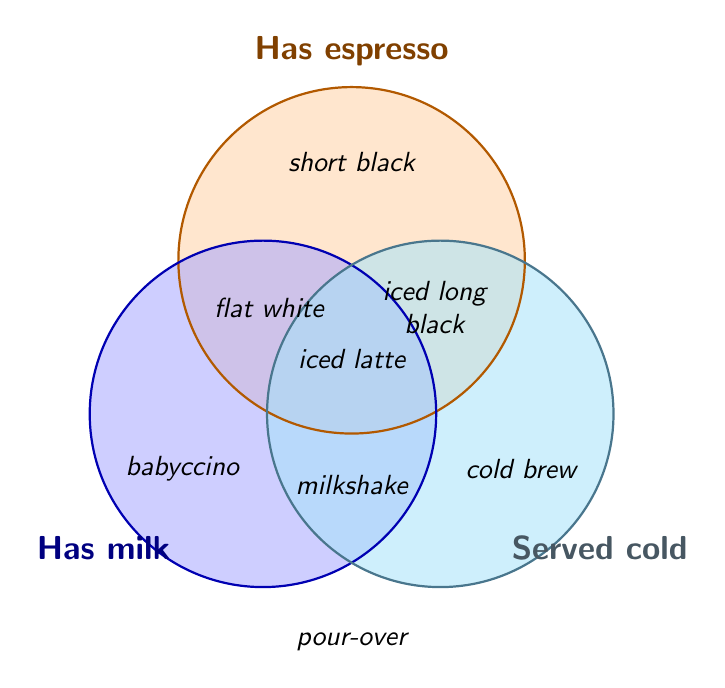
\begin{tikzpicture}[font=\sffamily]

% circle centres: espresso (top), milk (lower left), cold (lower right)
% radius 2.2, centres 1.3 from origin
\def\r{2.2}
\coordinate (E) at (0,1.3);
\coordinate (M) at (-1.126,-0.65);
\coordinate (C) at (1.126,-0.65);

% translucent fills so overlaps darken naturally
\fill[orange!35, opacity=0.55] (E) circle (\r);
\fill[blue!35,   opacity=0.55] (M) circle (\r);
\fill[cyan!35,   opacity=0.55] (C) circle (\r);

% outlines
\draw[orange!70!black, thick] (E) circle (\r);
\draw[blue!70!black,   thick] (M) circle (\r);
\draw[cyan!50!black,   thick] (C) circle (\r);

% set labels (outside each circle, on its outer side)
\node[font=\sffamily\bfseries\large, orange!50!black] at (0,3.95) {Has espresso};
\node[font=\sffamily\bfseries\large, blue!50!black]   at (-3.15,-2.35) {Has milk};
\node[font=\sffamily\bfseries\large, cyan!30!black]   at (3.15,-2.35) {Served cold};

% ---- drinks ----
% espresso only
\node[font=\sffamily\itshape] at (0,2.55) {short black};
% milk only
\node[font=\sffamily\itshape] at (-2.15,-1.35) {babyccino};
% cold only
\node[font=\sffamily\itshape] at (2.15,-1.35) {cold brew};
% espresso & milk (hot)
\node[font=\sffamily\itshape, align=center] at (-1.05,0.7) {flat white};
% espresso & cold
\node[font=\sffamily\itshape, align=center] at (1.05,0.7) {iced long\\black};
% milk & cold
\node[font=\sffamily\itshape] at (0,-1.55) {milkshake};
% all three
\node[font=\sffamily\itshape] at (0,0.05) {iced latte};
% outside everything
\node[font=\sffamily\itshape] at (0,-3.55) {pour-over};

\end{tikzpicture}
\end{document}